\section{第五回 フーリエ変換}
%-----------------------------------------------------------------------

\subsection{目的}
フーリエ変換の定義を覚え、フーリエ変換により、線形微分方程式が
代数方程式となることを理解する。さらに、逆フーリエ変換の実行には
複素積分が必要となることを理解する。

\subsection{解答}

\ans{16}{1}
積分の線形性より明らか。

\ans{16}{2}
フーリエ変換の定義より、
\begin{equation}
  \hat{f}(k) = \int_{-\infty}^{\infty} \!\!\! \diff x f(x) \e^{-ikx}
\end{equation}
部分積分を用いることで、
\begin{eqnarray}
  \hat{f}(k) &=& \int_{-\infty}^{\infty} \!\!\! \diff x f(x) \left( \frac{\e^{-ikx}}{-ik}\right)'\\
  &=&
  \left[
    f(x)  \frac{\e^{-ikx}}{-ik}
    \right]_{-\infty}^{\infty}
  + \frac{1}{ik}\int_{-\infty}^{\infty} \!\!\! \diff x f'(x) \e^{-ikx}\\
  &=& \frac{1}{ik}\int_{-\infty}^{\infty} \!\!\! \diff x f'(x) \e^{-ikx}
\end{eqnarray}
以上より、
\begin{equation}
  (ik) \hat{f}(k) = {\cal F}[f'(x)]
\end{equation}
以後、同様に繰り返すことで、
\begin{equation}
  (ik)^n \hat{f}(k) = {\cal F}[f^{(n)}(x)]
\end{equation}
を得る。

\ans{16}{3}
\begin{eqnarray}
  {\cal F}[f(x+a)] &=& \int_{-\infty}^{\infty} \!\!\! \diff x f(x+a) \e^{-ikx}\\
  &=& \int_{-\infty}^{\infty} \!\!\! \diff x f(x) \e^{-ik(x-a)}\\
  &=& \e^{ika} \int_{-\infty}^{\infty} \!\!\! \diff x f(x) \e^{-ikx}\\
  &=& e^{ika} \hat{f}(k)
\end{eqnarray}
ただし、途中で$x \rightarrow x-a$の変数変換を用いた。

\ans{16}{4}
フーリエ変換の定義より、
\begin{equation}
  \hat{f}(k) = \int_{-\infty}^{\infty} \!\!\! \diff x f(x) \e^{-ikx}
\end{equation}
両辺を$k$で形式的に微分すると、
\begin{eqnarray}
  \hat{f}'(k) &=& \int_{-\infty}^{\infty} \!\!\! \diff x (-ix) f(x) \e^{-ikx}\\
  &=& -i \int_{-\infty}^{\infty} \!\!\! x f(x) \e^{-ikx} \diff x\\
  &=& -i {\cal F}[x f(x)]
\end{eqnarray}
以上から、
\begin{equation}
  {\cal F}[x f(x)] = i \hat{f}'(k)
\end{equation}
同様に微分を繰り返せば、
\begin{equation}
  {\cal F}[x^n f(x)] = (i)^n \hat{f}^{(n)}(k)
\end{equation}
を得る。

\ans{16}{5}
フーリエ変換とたたみ込み積分の定義から、
\begin{eqnarray}
  {\cal F}[f*g] &=& \int_{-\infty}^{\infty} \diff x \e^{-ikx} \int_{-\infty}^{\infty} f(x-y)g(y)\diff y \\
  &=& \int_{-\infty}^{\infty} \diff y \e^{-iky} g(y) \int_{-\infty}^{\infty} \diff x \e^{-i(x-y)} f(x-y)\\
  &=& {\cal F}[g] {\cal F}[f]
\end{eqnarray}


\ans{17}{1}
\begin{eqnarray}
  \hat{f}(k) &=& \int_{-\infty}^{\infty} \!\!\! \diff x f(x) \e^{-ikx} \\
  &=& \int_{-a}^{a} \!\!\! \diff x \e^{-ikx} \\
  &=&
  \left[
    \frac{e^{ikx}}{-ik}
    \right]_{-a}^{a}\\
  &=& \frac{\e^{ika}-\e^{-ika}}{-ik}\\
  &=& \frac{2\sin ka}{k}
\end{eqnarray}

\ans{17}{2}
\begin{eqnarray}
  \hat{f}(k) &=& \int_{-\infty}^{\infty} \!\!\! \diff x f(x) \e^{-ikx} \\
  &=&
  \int_{-\infty}^{0} \!\!\! \diff x \e^{ax} \e^{-ikx}+
  \int_{0}^{\infty} \!\!\! \diff x \e^{-ax} \e^{-ikx}\\
  &=& \frac{1}{a-ik} + \frac{1}{a+ik} \\
  &=& \frac{2a}{a^2+k^2}
\end{eqnarray}

\ans{18}{1}
微分方程式全体をフーリエ変換すると、フーリエ変換の線形性より
\begin{equation}
  (ik)^2 \hat{y} - 2 (ik) \hat{y} = {\cal F}[\delta(x)]
\end{equation}
さて、デルタ関数のフーリエ変換は、
\begin{eqnarray}
  {\cal F}[\delta(x)] &=& \int_{-\infty}^{\infty} \!\!\! \diff x \delta(x) \e^{-ikx}\\
  &=& 1
\end{eqnarray}
以上より、
\begin{equation}
  (ik)^2 \hat{y} - 2 (ik) \hat{y} = 1
\end{equation}
整理すると、
\begin{equation}
  \hat{y}(k) = \frac{-1}{k^2+2ik}
\end{equation}
すなわち、{\bf フーリエ変換により線形微分方程式は代数方程式となる}。
これは後に学習するラプラス変換でも同様である。
ここで得られた$\hat{y}(k)$フーリエ逆変換すれば解$y(x)$が求められるが、
そのためには次の計算
\begin{equation}
  y(x) = \frac{1}{2 \pi} \int_{-\infty}^{\infty}\diff k \frac{-1}{k^2+2ik} \e^{ikx}
\end{equation}
を実行しなくてはならない。この積分には複素積分の知識が必要となる。

\ans{18}{2}
前問と同様にフーリエ変換を行うと、
\begin{equation}
  (ik)^2 \hat{y} - \hat{y} = {\cal F}[\e^{-ax^2}]
\end{equation}
となる。したがって、${\cal F}[\e^{-ax^2}]$を計算しなくてはいけない。
\begin{eqnarray}
  {\cal F}[\e^{-ax^2}] &=& \int_{-\infty}^{\infty}\diff x \e^{-ax^2} \e^{-ikx}\\
  &=& \int_{-\infty}^{\infty}\diff x \exp({-ax^2-ikx})\\
  &=& \int_{-\infty}^{\infty}\diff x \exp\left( -a \left(x+\frac{ik}{2}\right)^2 - \frac{k^2}{4a} \right)\\
  &=& \exp(-{\frac{k^2}{4a}})  \int_{-\infty}^{\infty}\diff x \exp\left( -a (x+\frac{ik}{2})^2 \right)\\
  &=& \sqrt{\frac{\pi}{a}} \exp(-{\frac{k^2}{4a}})
\end{eqnarray}
すなわち、{\bf ガウス分布のフーリエ変換はガウス分布となる}。
ただし、ガウス分布の広がり(分散)が逆になっていることに注意しよう。
すなわち、実空間でなだらかなガウス分布は、波数空間では狭い分布となる(逆もまたしかり)。
これはガウス分布だけでなく、フーリエ変換一般に言える性質である。

ちなみに、ここでフーリエ変換により微分方程式が代数方程式になったのは、
元の方程式が線形だったからである。
すなわち、{\bf 非線形微分方程式をフーリエ変換しても代数方程式にはならない}。
フーリエ変換はものの見方を変えているだけであって、
難しい問題は、変換しても難しいままとなるのである。

\subsection{解説}

問題で、
$$
  y''(x) - y(x) = \delta(x)
$$
の形の微分方程式を扱った。この解が求まると、一般の関数$f(x)$が含まれた
微分方程式
$$
  g''(x) - g(x) = f(x)
$$
の解を$y(x)$を使って表現できる。

まず、$y(x)$のフーリエ変換を考えると、
\begin{equation}
  {\cal F}[y] = -\frac{1}{k^2+1}
\end{equation}
また、$g(x)$のフーリエ変換は
\begin{equation}
  {\cal F}[g] = -\frac{1}{k^2+1} {\cal F}[f]
\end{equation}
したがって、
\begin{equation}
  {\cal F}[g] = {\cal F}[y] {\cal F}[f]
\end{equation}
左辺はたたみ込み積分のフーリエ変換として表現できるから、
\begin{equation}
  {\cal F}[g] = {\cal F}[y*f(x)]
\end{equation}
もとに戻すと、
\begin{equation}
  g(x) = \int_{-\infty}^{\infty}f(s) y(x-s)  \diff s
\end{equation}
以上より、一般の$f(x)$を含む微分方程式の解を得た。
あとはそれぞれの場合において$f(x)$を代入し、積分を実行すれば
$g(x)$を得ることができる。このように、デルタ関数は
たたみ込み積分と密接な関係を持つ。このことは後に学ぶ
ラプラス変換でより明らかとなる。


%-----------------------------------------------------------------------
\newpage
\section{第六回 複素積分とローラン展開}
%-----------------------------------------------------------------------

\subsection{目的}

複素関数の正則性および複素積分の基礎について学ぶ。
また、留数定理の準備として、ローラン展開について学ぶ。

\subsection{解答}

\ans{19}{1}

$z_0 = x_0 + i y_0$、
$x - x_0 = \Delta x$、
$y - y_0 = \Delta y$としよう。
$f(z)$の実部を$u(x,y)$、虚部を$v(x,y)$とすると、
$$
  \lim_{\Delta z \rightarrow 0} \frac{f(z+\Delta z) - f(z)}{\Delta z}
  =
  \lim_{\Delta z \rightarrow 0} \frac{u(x+\Delta z,y+\Delta y) - u(x,y)}{\Delta x + i \Delta y}
  + \lim_{\Delta z \rightarrow 0} i \frac{v(x+\Delta z,y+\Delta y) - v(x,y)}{\Delta x + i \Delta y}
$$
ここで、まず$y$軸をあわせて、$x$軸から近づく場合を考える。
すると、$\Delta y = 0$であるから、
\begin{eqnarray}
  \lim_{\Delta z \rightarrow 0} \frac{f(z+\Delta z) - f(z)}{\Delta z}
  &=&
  \lim_{\Delta x \rightarrow 0} \frac{u(x+\Delta x,y) - u(x,y)}{\Delta x}
  + \lim_{\Delta x \rightarrow 0} i \frac{v(x+\Delta x,y) - v(x,y)}{\Delta x}\\
  &=&
  \frac{\partial u}{\partial x} + i \frac{\partial v}{\partial x}
\end{eqnarray}
同様に、$\Delta x = 0$とすると、
\begin{eqnarray}
  \lim_{\Delta z \rightarrow 0} \frac{f(z+\Delta z) - f(z)}{\Delta z}
  &=&
  \lim_{\Delta y \rightarrow 0} \frac{u(x,y+\Delta y) - u(x,y)}{i\Delta y}
  + \lim_{\Delta y \rightarrow 0} i \frac{v(x,y+\Delta y) - v(x,y)}{i\Delta y}\\
  &=&
  -i \frac{\partial u}{\partial y} + \frac{\partial v}{\partial y}
\end{eqnarray}
を得る。分母に$i$があることに注意。
これらが一致しなくてはならないのだから、実部と虚部を比較すると、
コーシー・リーマンの関係式、
$$
  \frac{\partial u}{\partial x} = \frac{\partial v}{\partial y},
  \frac{\partial u}{\partial y} = -\frac{\partial v}{\partial x}
$$
を得る。

\ans{19}{2}

$z = x+ iy$とし、$z^2$の実部と虚部を求めると、
\begin{eqnarray}
  z^2 &=& (x+iy)^2\\
  &=& x^2 - y^2 +  2ixy
\end{eqnarray}
したがって、$u = x^2 - y^2$、$v = 2xy$
である。
それぞれ$x$および$y$で偏微分すればコーシー・リーマンの関係式を満たすことがわかる。
一般に、実部や虚部、絶対値や複素共役など、あらわに複素数を操作する関数以外の関数、
すなわち実数関数の$x$をそのまま$z$で置き換えた関数はほぼ正則であり、
その実部と虚部はコーシー・リーマンの関係式を満たすと思ってよい。

\ans{19}{3}
前問と同様に
$z = x+ iy$とし、$z^2$の実部と虚部を求めると、
\begin{eqnarray}
  z\bar{z} &=& (x+iy)(x-iy)\\
  &=& x^2 + y^2
\end{eqnarray}
したがって、この関数はつねに実数値をとるので、
実部と虚部の関係式であるコーシー・リーマンの関係式は満たさない。
なお、$z \bar{z} = |z|^2$、すなわち$z$の絶対値であることにも注意しておこう。

\ans{20}{1}

$z = (1+i)t$とおけば、積分は$t$をパラメータとして、
$$
  \int z^2 \diff z = \int_0^1 (1+i)^3 t^2  \diff t
$$
とあらわすことができる($\diff z = (1+i) \diff t$に注意せよ)。
これは簡単に積分できて、
$$
  (1+i)^3 \int_0^1 t^2  \diff t = \frac{(1+i)^3}{3}
$$
すなわち、単に$z$を実数の場合と同様に
$$
  \int_0^{1+i} z^2 \diff z = \left[ \frac{z^3}{3}  \right]_0^{1+i}
$$
とするのと同じ結果が得られた。
{\bf これは今回考えた関数が積分範囲で正則であったからである。}
一般に、積分範囲で正則な複素関数は、実数と同様に積分でき、
その値は積分経路に依存しない(積分値は始点と終点のみに依存する)。

\ans{20}{2}
点$a$を中心とする半径$r$の円は、極座標を用いて
$z = a + r\e^{i\theta} ~(0 \le \theta < 2\pi)$とあらわすことができる。
$\diff z = ri \e^{i\theta} \diff \theta$に注意すると、
もとの積分は$\theta$をパラメータとして、
\begin{equation}
  \oint (z-a)^n \diff z = i r^{n+1} \int_0^{2\pi} \e^{i(n+1)\theta} \diff \theta
\end{equation}
と表せる。
ここで、$n = -1$の場合とそうでない場合を分けて考えると、
\begin{equation}
  \oint (z-a)^n \diff z =
  \left\{
  \begin{array}{cccc}
    i r^{n+1} \left[ \displaystyle\frac{\e^{i(n+1)\theta}}{i(n+1)} \right]_0^{2\pi} & = & 0      & (n \neq -1) \\
    i \left[ \theta  \right]_0^{2\pi}                                               & = & 2\pi i & (n=-1)
  \end{array}
  \right.
\end{equation}
を得る。すなわち、$z^n$の形を特異点周りに周回積分した場合、
$1/z$以外はすべて$0$となる。これは重要な結果である。
後に述べるローラン展開において、適当な周回積分に寄与する項は
$c_{-1}$のみということを意味する。したがって、この項の値さえ
わかれば積分値が求められる。これも複素関数の正則性という
(関数にとって)厳しい条件からの帰結である。

\ans{21}{1}

$|z|<1$の場合、例に挙げられた展開で$-z$を代入すればよいから、
\begin{eqnarray}
  \frac{1}{z-1} &=& - \frac{1}{1-z}\\
  &=& -(1 + z + z^2 + \cdots + z^n + \cdots) \\
  &=& -\sum_{n=0}^{\infty} z^n
\end{eqnarray}

$|z|>1$の場合、$|1/z|<1$に注意すれば、
\begin{eqnarray}
  \frac{1}{z-1} &=& \frac{1}{z} \frac{1}{1 - 1/z}\\
  &=& z^{-1}
  \left(
  1 + z^{-1}+ z^{-2}+ \cdots
  \right)\\
  &=& \sum_{n=1}^{\infty} z^{-n}
\end{eqnarray}
すなわち、{\bf ローラン展開は同じ中心でも範囲によって係数が異なる}。
正確に言うと、範囲が新たな特異点をまたぐときに値が変わる。
これがなぜかは留数定理を学ぶときに明らかになるだろう。

\ans{21}{2}
まず、$f(z)$を部分分数分解すると、
\begin{equation}
  f(z) = \frac{1}{z(z-1)} = \frac{1}{z-1} - \frac{1}{z}
\end{equation}
あとは前問と同様に解くことができる。

\subsection{解説}

\subsubsection{正則性}
複素関数$f(z)$が、ある領域$D$のすべての点で微分可能であるとき、
$f(z)$は$D$において{\bf 正則 (holomorphic)}であるという。
複素関数$f(z)$がある点で微分可能であるためには、その実部と虚部に
コーシー・リーマンの関係式が成り立ってなくてはいけない。
この関係式をさらに$x$,$y$で偏微分してみよう。
\begin{eqnarray}
  \frac{\partial^2 u}{\partial x^2} &=& \frac{\partial^2 v}{\partial x \partial y}\\
  \frac{\partial^2 u}{\partial y^2} &=& - \frac{\partial^2 v}{\partial x \partial y}
\end{eqnarray}
すなわち、
\begin{equation}
  \Delta u = 0
\end{equation}
が成り立つことがわかる。ここで$\Delta \equiv \partial^2/\partial x^2 + \partial^2/\partial y^2$は
ラプラシアンである。
同様に、虚部である$v$についても
\begin{equation}
  \Delta v = 0
\end{equation}
が成り立つ。ラプラシアンを演算して0となる関数を
{\bf 調和関数 (Harmonic function)}であるという。
複素関数$f(z)= u(x,y) + i v(x,y)$が正則であるためには、
実部$u(x,y)$、虚部$v(x,y)$がそれぞれ調和関数でなくてはならない。
したがって、実数関数の微分可能性よりも厳しい条件が必要であり、
これが複素関数論の豊富な応用を生み出す。

複素関数が正則でないとは、たとえば$1/z$のように$\lim z \rightarrow 0$で無限大になってしまうものや、
$Re z$や$z \bar{z}$のように実部と虚部をあらわに操作する関数などがある。
しかし、本ゼミにおいては実積分のために複素積分を用いるのが目的なので
実用上は値が無限大になる点においては正則でないと覚えておけば良い。

\subsubsection{特異点}

関数$f(z)$が、点$a$では正則ではないが、その点の近傍に$f(z)$が正則であるような
点が存在するとき、$a$を$f(z)$の{\bf 特異点 (singular point)}と呼ぶ。
特に、$a$の任意の近傍に特異点が無い場合、$a$を孤立特異点と呼ぶ。
物理数学で扱われる特異点はほぼすべて孤立特異点である

点$a$が関数$f(z)$の孤立特異点である場合、そのまわりで、
\begin{equation}
  f(z) = \sum_{n=-\infty}^{\infty} c_n(z-a)^n
\end{equation}
と展開できる。これを{\bf ローラン(Laurent)展開}と言う。
このとき、$n\ge 0$の項、すなわち、
$\sum_{n=0}^{\infty} c_n(z-a)^n$は点$a$においても正則であるから、
$f(z)$の特異性は、残りの項
$\sum_{n=-\infty}^{-1} c_n(z-a)^n$
によると考えられる。この項をローラン展開の主要部と呼ぶ。

まず、主要部が無い場合は、点$a$を除きうる特異点と呼び、
$\lim_{z\rightarrow a} f(z)$の値を適当に再定義すれば
$f(z)$は$a$において正則となる。

主要部が無限項である場合、$a$を{\bf 真性特異点 (essential singularity)}と呼ぶ。
たとえば$\e^{1/z}$は、原点が真性特異点となる。

最後に主要部が有限項である場合、点$a$を{\bf 極 (pole)}と呼ぶ。
物理数学で扱うのは主にこの極である。特に、主要部の最高次数が$k$で
ある場合、$a$を$f(z)$の{\bf k位の極}と呼ぶ。


%-----------------------------------------------------------------------
\newpage
\section{第七回 留数定理とその応用}
%-----------------------------------------------------------------------

\subsection{目的}

留数定理を用いた複素積分と、その応用として実定積分の計算方法を学ぶ。

\subsection{解答}

\ans{22}{1}
$\e^{z}$は正則な関数であるから、公式で$f(z)=\e^z$、$a=-1$と置けばよい。
\begin{eqnarray}
  \frac{1}{2\pi i} \int_{|z|=2} \frac{\e^z}{z+1} &=& f(-1)\\
  &=& e^{-1}
\end{eqnarray}
すなわち、
\begin{equation}
  \int_{|z|=2} \frac{\e^z}{z+1} = 2\pi i e^{-1}
\end{equation}
ここで、積分路が囲む範囲$|z|<2$に、特異点$z=-1$が含まれることに注意しよう。
積分路が特異点を囲まなければ関数$\e^z/(z+1)$は正則となるので
周回積分は$0$である。

\ans{22}{2}
まず、部分分数分解を行う。
\begin{equation}
  \frac{z}{z^2+1} = \frac{1}{2} \left( \frac{1}{z+i} + \frac{1}{z-i} \right)
\end{equation}
コーシーの積分定理から、
\begin{eqnarray}
  \int_{|z|=2} \frac{1}{z+i} \diff z & =& 2 \pi i \\
  \int_{|z|=2} \frac{1}{z-i} \diff z & =& 2 \pi i \\
\end{eqnarray}
であるから、
\begin{equation}
  \int_{|z|=2} \frac{1}{z^2+1} = \frac{2\pi i + 2\pi i}{2} = 2 \pi i
\end{equation}

\ans{23}{1}
$f(z) = \e^{3z}$とおけば、コーシーの積分公式より、
\begin{equation}
  \frac{1}{2\pi i} \int_{|z|=3} \frac{f(z)}{(z-2)^2} = f'(2) = 3\e^{6}
\end{equation}
以上から、
\begin{equation}
  \int_{|z|=3} \frac{\e^{3z}}{(z-2)^2} = 6 \pi i \e^{6}
\end{equation}

\ans{23}{2}
まず注意したいのは、関数$\displaystyle \frac{1}{z^2(z-3)}$は
特異点として$z=0,3$を持つが、積分範囲$|z|=1$の中にあるのは$z=0$のみである。
したがって、関数$1/(z-3)$は積分領域で正則であるから、
$f(z) = 1/(z-3)$と置けば、
\begin{equation}
  \frac{1}{2\pi i} \int_{|z|=1} \frac{f(z)}{z^2} = f'(0) = - \frac{1}{9}
\end{equation}
したがって、
\begin{equation}
  \int_{|z|=1} \frac{1}{z^2(z-3)} =- \frac{2 \pi i}{9}
\end{equation}
このように、特異点のうち積分に寄与するのは、閉曲線の内部にあるもののみである。
これは、$|z|<3$と、$|z|>3$の二つの範囲で$\displaystyle \frac{1}{z^2(z-3)}$をローラン展開すればより明確に理解できよう。


\ans{24}{1}
まず、$\e^{iz}$は(無限遠を除いた)すべての領域で正則であることに注意しよう。
したがって特異点は$z = \pm i a$である。
部分分数分解すると、
\begin{equation}
  \frac{\e^{iz}}{z^2+a^2} = \frac{\e^{iz}}{2ia}
  \left(
  \frac{1}{z-ia} - \frac{1}{z+ia}
  \right)
\end{equation}
となる。
$z=ia$の周りで周回積分すると、
\begin{equation}
  \frac{1}{2\pi i} \int_{|z-ia|=\sigma} \frac{\e^{iz}}{2ia}
  \left(
  \frac{1}{z-ia} - \frac{1}{z+ia}
  \right)
  = \frac{\e^{-a}}{2ia}
\end{equation}
以上から、
\begin{equation}
  \mbox{Res} f(ia) = \frac{\e^{-a}}{2ia}
\end{equation}
同様に、$z=-ia$の周りで周回積分すれば、
\begin{equation}
  \mbox{Res} f(-ia) = - \frac{\e^{a}}{2ia}
\end{equation}
を得る。

{\bf 別解}\\
留数とは、ローラン展開したときの係数の$c_{-1}$そのものである。
したがって、$f(z)$が$a$を一位の極として持つなら、
\begin{equation}
  f(z) = c_{-1} (z-a)^{-1} + c_0 + c_1 (z-a) + c_2 (z-a)^2 + \cdots
\end{equation}
と展開されるはずである。
そこで、$f(z)(z-a)$をかけてから、極限$\lim z \rightarrow a$を考えると、
\begin{equation}
  \lim_{z \rightarrow a} f(z)(a-z) = c_{-1}
\end{equation}
となり、これは求める留数である。

この方法を問題に適用すると、
\begin{equation}
  \mbox{Res} f(ia) = \lim_{z \rightarrow ia} \left( (z-ia) \frac{\e^{iz}}{z^2+a^2} \right)
  = \frac{\e^{-a}}{2ia}
\end{equation}
\begin{equation}
  \mbox{Res} f(-ia) = \lim_{z \rightarrow -ia} \left( (z+ia) \frac{\e^{iz}}{z^2+a^2} \right)
  = -\frac{\e^{a}}{2ia}
\end{equation}
とすぐに求めることができる。
物理数学において複素積分は計算を簡単に行うための便法であるので、
複素積分自体もなるべく簡単に計算ができるように工夫したい。
そのためには典型的なパターンをいくつか覚える必要があるが、今回の例はその一つである。
他には$1/(1-z)$のテイラー展開を利用するものなどがある。

\ans{24}{2}
特異点は$\e^{i \pi /4}$、$\e^{i 3\pi /4}$、$\e^{-i \pi /4}$、$\e^{-i 3\pi /4}$の4つで、いずれも一位の極である。
部分分数展開しても良いが、前問の別解を使うほうが便利である。

$z = \e^{i \pi /4}$における留数は
\begin{equation}
  \mbox{Res} f(\e^{i \pi /4}) = \lim_{z \rightarrow \e^{i \pi /4}} \left( \frac{z-\e^{i \pi /4}}{z^4+1} \right)
  = \frac{\exp{(-3\pi i/4})}{4}
\end{equation}
ただし、$f(0)=g(0)=0$の時、
\begin{equation}
  \lim_{x\rightarrow 0} \frac{f(x)}{g(x)} = \frac{f'(x)}{g'(x)}
\end{equation}
を用いた(ロピタルの定理)。
他の留数も同様に求められる。

\ans{25}{1}
まず、$x^4+1$は偶関数であるから、
\begin{equation}
  \int_0^{\infty} \frac{1}{x^4+1} \diff x = \frac{1}{2} \int_{-\infty}^{\infty}  \frac{1}{x^4+1} \diff x
\end{equation}
として、以下の図のような積分路$C$を考える。
\begin{figure}[htbp]
  \begin{center}
    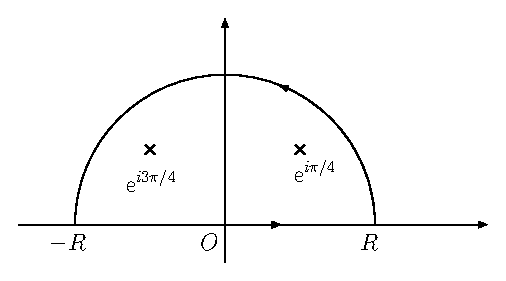
\includegraphics[width=.5\linewidth]{fig/z_int2.eps}
  \end{center}
  \caption{
    半円の積分路。$R$は無限大にする。
  }
  \label{fig_z_int2}
\end{figure}
ここで、$\lim R \rightarrow \infty$の極限で、半円の部分の積分の寄与は$0$となる(解説参照)。
したがって、
\begin{equation}
  \int_{-\infty}^{\infty} \frac{1}{x^4+1} \diff x = \lim_{R \rightarrow \infty} \int_C \frac{1}{z^4+1} \diff z
\end{equation}
ここで、積分路の内部にある特異点は$z = \e^{i\pi/4},\e^{i3\pi/4}$の二つであるから、
\begin{eqnarray}
  \int_C \frac{1}{z^4+1} \diff z &=& 2 \pi i \left( \mbox{Res} f(\e^{\pi i/4}) +\mbox{Res} f(\e^{3\pi i/4})  \right)\\
  &=& 2 \pi i \left(  \frac{\exp{(-3\pi i /4})}{4} + \frac{\exp{(-9 \pi i /4})}{4}  \right)\\
  &=& 2 \pi i \left(  \frac{\e^{\pi i/4}-\e^{- \pi i/4}}{4}  \right)\\
  &=& \pi \sin \frac{\pi}{4}
\end{eqnarray}
以上より、
\begin{equation}
  \int_0^{\infty} \frac{1}{x^4+1} \diff x = \frac{\pi}{2} \sin \frac{\pi}{4} = \frac{\pi}{2\sqrt{2}}
\end{equation}

\ans{25}{2}
$f(z) = \e^{ikz}/(z^2+1)$とし、以下の複素積分を考える。
\begin{equation}
  \int_C \frac{e^{ikz}}{z^2+1} \diff z
\end{equation}
まず、$f(z)$の上半面内の特異点は$z=i$のみであるので、
\begin{eqnarray}
  \int_C \frac{e^{ikz}}{z^2+1} \diff z &=& 2\pi i ~\mbox{Res} f(i)\\
  &=& 2\pi i \left( \frac{\e^{-k}}{2i} \right) \\
  &=& \pi \e^{-k}
\end{eqnarray}
以上から、
\begin{equation}
  \int_{-\infty}^{\infty} \frac{\cos kx}{x^2+1} \diff x =
  \mbox{Re} \int_C \frac{\e^{ikz}}{z^2+1} \diff z = \pi \e^{-k}
\end{equation}

\subsection{解説}

\subsubsection{コーシーの積分定理}

複素関数が微分可能であるとき、その実部と虚部には
強い制限(コーシー・リーマンの関係式)が課せられるのであった。
その帰結として、以下のコーシーの積分定理が成り立つ。

関数$f(z)$が領域$D$で正則であるとする。$C$は$D$内の単一閉曲線で、
$C$の内部が$D$の点のみであるとき、
\begin{equation}
  \int_C f(z) \diff z = 0
\end{equation}
が成り立つ。すなわち、{\bf 正則な関数を周回積分すると値が$0$となる}。
この積分定理と関数の正則性から、以下のコーシーの積分公式が導かれる。

関数$f(z)$は領域$D$であり、$C$は内部に領域$D$の点のみを持つ単一閉曲線である。
このとき、$C$内の点$a$について、以下の公式が成り立つ。
\begin{equation}
  f(a) = \frac{1}{2\pi i} \int_C \frac{f(z)}{z-a} \diff z \label{eq_cauchy1}
\end{equation}
これは、$C$の内部の任意の点$a$での値$f(a)$が$C$上の$f(z)$の値だけで決まる、
すなわち、{\bf 境界の値からその内部の値がすべて決まることを意味している}。
さらに以下の公式が成り立つ(これもコーシーの積分公式と呼ばれる)。
\begin{equation}
  f^{n}(a) = \frac{n!}{2\pi i} \int_C \frac{f(z)}{(z-a)^{n+1}} \diff z  \label{eq_cauchy2}
\end{equation}
すなわち、{\bf 積分の値が微分から求められる}。
これらの性質はすべて、複素関数が微分可能(正則)であるという条件が厳しいからである。
ここで、式(\ref{eq_cauchy2})は、式(\ref{eq_cauchy1})を形式的に左右$a$で微分した形に
なっていることに注意しよう。

さて、なぜコーシーの積分定理が成り立つか考えよう。
まず、$(z-a)^n$を$a$の周りに周回積分すると、その半径にかかわらず
\begin{eqnarray}
  \int_{|z-a|=r} (z-a)^n \diff z=
  \left\{
  \begin{array}{ccc}
     & 0      & (n \neq -1) \\
     & 2\pi i & (n = -1)
  \end{array}
  \right.
\end{eqnarray}
となるのであった。
また、$f(z)$が考えている領域で正則であるならば、
\begin{equation}
  f(z) = f(a) + f'(a) (z-a) + \frac{f''(a)(z-a)^2}{2} + \cdots
\end{equation}
と$a$の周りでテイラー展開できる。
したがって、
\begin{equation}
  \frac{f(z)}{z-a} = \frac{f(a)}{z-a} + f'(a) + \frac{f''(a)(z-a)}{2} + \cdots
\end{equation}
となるから\footnote{%
  これは$f(z)/(z-a)$の$a$におけるローラン展開である。
}、周回積分すれば、$1/(z-a)$の係数のみが残るので、
\begin{equation}
  \int_C \frac{f(z)}{z-a} \diff z = 2\pi i f(a)
\end{equation}
と、コーシーの積分公式を得た。
同様に$f(z)/(z-a)^{n+1}$の展開を考えることで公式(\ref{eq_cauchy2})も得ることができる。
記憶する便法として、$a$による形式的な微分をしても良いが、
ローラン展開をして$1/(z-a)$の係数を求めているのが本質であることを理解して欲しい。

\subsubsection{実定積分への応用}

複素積分は、実関数の定積分の値を求めるのに用いることができる。
複素積分を用いるのは、原始関数は求められないが、ある特別な区間においては定積分の値が求まる場合と、
原始関数が求められる場合でも複素積分を用いたほうが計算が簡単である場合がある。

物理数学において出てくる積分のパターンには、まず
\begin{equation}
  \int_{-\infty}^{\infty} \frac{f(x)}{g(x)} \diff x
\end{equation}
というタイプがある。ただし$f(x)$、$g(x)$はそれぞれ$m$次と$n$次の多項式であり、
$m\le n + 2$を満たすとする。さらに$g(x)=0$は実数解を持たないとする。

まず、前者の場合は、
積分路$C$を図\ref{fig_z_int2}のように半円型にとり、
複素積分
\begin{equation}
  \lim_{R \rightarrow \infty}\int_C \frac{f(z)}{g(z)} \diff z
\end{equation}
を考えるのが定石。ここで、円周の積分は半径$R$を無限大にすれば$0$となる。
それは、$f(z)$が$m$次、$g(z)$が$n$次の多項式であり、
$m\le n + 2$を満たすことから、$\lim |z| \rightarrow \infty$において
\begin{equation}
  \left| \frac{f(z)}{g(z)} \right| \leq \frac{1}{|z|^2}
\end{equation}
を満たす。
したがって、半径$R$の円周上$C_1$において
\begin{eqnarray}
  \int_{C_1} \frac{f(z)}{g(z)} \diff z &\leq& \int_{C_1} \left| \frac{f(z)}{g(z)} \right| \diff z \\
  &\leq& \int_{C_1}  \frac{1}{|z|^2} \diff z\\
  &= & \frac{1}{R}
\end{eqnarray}
以上から、$R \rightarrow \infty$の極限で、円周上の積分の寄与が$0$になるのである。
逆に、$|z| \rightarrow \infty$の極限に対して、$1/z^2$より早く$0$になる
複素関数でなければ、円周上の積分を$0$とおいてはいけない。

さて、円周の積分が$0$であるから、「実軸の積分」は「実軸を含む周回積分」と等しいことがわかる。
ここで、複素関数の周回積分は留数定理で簡単に値を求めることができる。
以上より実関数の定積分が複素積分により求められるのである。

複素積分を使った実定積分には、もう一つ
\begin{equation}
  \int_{-\infty}^{\infty} \frac{f(x)\cos(kx)}{g(x)} \diff x
\end{equation}
というパターンがある。ただし、$f(x)$と$g(x)$
それぞれ$m$次と$n$次の多項式であり、
$m\le n + 1$を満たすとする。さらに$g(x)=0$は実数解を持たないとする。

これは複素関数$F(z)$として、
\begin{equation}
  F(z) =  \frac{f(z) \e^{ikz}}{g(z)}
\end{equation}
を考えるのが定石である。
これについて複素積分を実行し、後で実部をとればよい。$\sin$の場合も同様に積分後に虚部を取る。

%-----------------------------------------------------------------------
\newpage
\section{第八回 フーリエ逆変換とジョルダンの補題}
%-----------------------------------------------------------------------

\subsection{目的}

フーリエ逆変換を行う際、複素積分の積分路をどのように取るべきかを学ぶ。

\subsection{解答}

\ans{26}{1}

フーリエ変換の定義より、
\begin{eqnarray}
  \hat{f}(k) &=& \int_{-\infty}^{\infty} f(x) \e^{-ikx} \diff x \\
  &=& \int_{-a}^{a} \e^{-ikx} \diff x \\
  &=& \left[ \frac{\e^{-ikx}}{-ik}  \right]_{-a}^a\\
  &=& \frac{1}{ik} \left( \e^{ika} - \e^{-ika} \right)
\end{eqnarray}

\begin{figure}[htbp]
  \begin{center}
    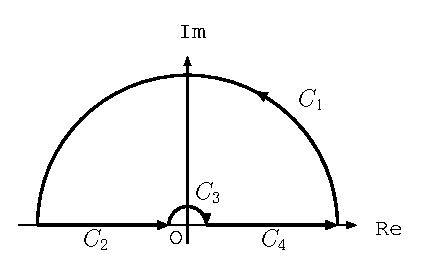
\includegraphics[width=.5\linewidth]{fig/jordan2.eps}
  \end{center}
  \caption{
    複素積分を行うための積分路。
    全体の積分路$C = C_1+C_2+C_3+C_4$は、積分路に特異点が無いから$0$。
    $(x+a)>0$であれば、十分大きな半径のとき$C_1=0$となる。
    また、$C_3$は、半径$0$の極限で$-\pi i $であり、
    求めたい積分は
    $
      \int_{-\infty}^{\infty} = \int_{C_2}+\int_{C_4} = -\int_{C_3}
    $
    から求まる。$(x+a)<0$の場合は下半面を回らなくてはいけない。
  }
  \label{fig_jordan2}
\end{figure}

\ans{26}{2}
逆フーリエ変換の定義から、
\begin{eqnarray}
  f(x) &=& \frac{1}{2\pi} \int_{-\infty}^{\infty} \hat{f}(k) \e^{ikx} \diff k \\
  &=& \frac{1}{2\pi i}\int_{-\infty}^{\infty} \left( \frac{\e^{i(x+a)k}}{k} - \frac{\e^{i(x-a)k}}{k} \right) \diff k
\end{eqnarray}
まず、第一項の積分を計算する。$x+a>0$の場合、
積分路$C$を図\ref{fig_jordan2}
$C = C_1 + C_2 + C_3 + C_4$のように取る。
$C$の中には極が無いから、
\begin{equation}
  \int_{C} \frac{\e^{i(x+a)z}}{z} \diff z = 0
\end{equation}
ジョルダンの補題より大きな半径を取れば$C_1= 0$である。
また、積分路$C_3$は、一位の極を時計回りに半分だけ回っているから
\begin{equation}
  \int_{C_3} \frac{\e^{i(x+a)z}}{z} \diff z = - \pi i
\end{equation}
である。以上から、
\begin{eqnarray}
  \int_{C_1+C_2+C_3+C_4} \frac{\e^{i(x+a)k}}{k} \diff k &= &0 \\
  \int_{C_2+C_4} \frac{\e^{i(x+a)k}}{k} \diff k - \pi i &= &0 \\
  \therefore \int_{-\infty}^{\infty} \frac{\e^{i(x+a)k}}{k} \diff k &=& \pi i
\end{eqnarray}
同様に、$x+a <0$の時には、
\begin{equation}
  \int_{C_2} \frac{\e^{i(x+a)z}}{z} \diff z = - \pi i
\end{equation}
となる。

まとめると、
\begin{equation}
  \int_{-\infty}^{\infty} \frac{\e^{i(x+a)k}}{k} \diff k =
  \left\{
  \begin{array}{cc}
    \pi i  & \quad (x > -a) \\
    -\pi i & \quad (x < -a)
  \end{array}
  \right.
\end{equation}
積分の第二項も同様に、
\begin{equation}
  \int_{-\infty}^{\infty} \frac{\e^{i(x-a)k}}{k} \diff k =
  \left\{
  \begin{array}{cc}
    \pi i  & \quad (x>a) \\
    -\pi i & \quad (x<a)
  \end{array}
  \right.
\end{equation}

以上をまとめると、
\begin{equation}
  f(x) = \left\{
  \begin{array}{cc}
    0 & \quad x < -a        \\
    1 & \quad -a \leq x < a \\
    0 & \quad a \leq x
  \end{array}
  \right.
\end{equation}
となり、確かに元の関数に一致する。

\ans{27}{1}

全体をフーリエ変換すると、
\begin{equation}
  (ik)^2 \hat{f} - \hat{f} = {\cal F}[\e^{-|x|}]
\end{equation}
ここで、
\begin{eqnarray}
  {\cal F}[\e^{-|x|}] & =&
  \int_{-\infty}^{\infty} \e^{-|x|} e^{-ikx} \diff x\\
  &=&
  \int_{-\infty}^{0} \e^{x} e^{-ikx} \diff x +
  \int_{0}^{\infty} \e^{-x} e^{-ikx} \diff x \\
  &=& \frac{1}{1-ik} + \frac{1}{1+ik}\\
  &=& \frac{2}{1+k^2}
\end{eqnarray}
以上から、
\begin{equation}
  \hat{f}(k) = - \frac{2}{(1+k^2)^2}
\end{equation}

\ans{27}{2}

逆フーリエ変換の定義より、
\begin{equation}
  f(x) = - \frac{1}{2\pi} \int_{-\infty}^{\infty}  \frac{\e^{ikx}}{(1+k^2)^2} \diff k
\end{equation}
$x>0$のとき、複素平面の上を通る半円を積分路とすると、
\begin{equation}
  \int_{-\infty}^{\infty}  \frac{\e^{ikx}}{(1+k^2)^2} \diff k
  = \int_C  \frac{\e^{ixz}}{(1+z^2)^2} \diff z
\end{equation}
このとき、積分路の中に、2位の極$z = i$があるから、
$F(z) = \displaystyle \frac{2 \e^{ixz}}{(z+i)^2}$とすれば、
\begin{eqnarray}
  \int_C  \frac{\e^{ixz}}{(1+z^2)^2} \diff z &=& \int_C  \frac{F(z)}{(z-i)^2} \diff z \\
  &=& 2 \pi i F'(i) \\
  &=& \frac{2\pi (1+x)}{2} \e^{-x}
\end{eqnarray}
すなわち、
\begin{equation}
  f(x) = - \frac{(1+x)}{2} \e^{-x}
\end{equation}

同様に、$x<0$のときは
\begin{equation}
  f(x) = - \frac{(1-x)}{2} \e^{x}
\end{equation}

まとめると、
\begin{equation}
  f(x) = - \frac{(1+|x|)}{2} \e^{-|x|}
\end{equation}

\ans{27}{3}

$x>0$のとき、
\begin{eqnarray}
  f(x) &=& -\frac{(1+x)}{2}e^{-x}\\
  \frac{\diff}{\diff x} f(x) &=& \frac{x}{2}e^{-x}\\
  \frac{\diff^2}{\diff x^2}  f(x) &=& \frac{(1-x)}{2}e^{-x}\\
\end{eqnarray}
以上から、
\begin{equation}
  \frac{\diff^2}{\diff x^2}  f(x) - f(x) = \e^{-x}
\end{equation}
$x<0$の場合も同様。

\subsection{解説}

関数$f(x)$のフーリエ変換$\hat{f}(k)$が存在するためには、積分
\begin{equation}
  \int_{-\infty}^{\infty} |f(x)|  \diff x
\end{equation}
が有限でなくてはならない。これを{\bf 絶対可積分}であるという。
フーリエ変換が可能である条件は、$f(x)$が区分的に滑らかで、
絶対可積分であることである。

さて、フーリエ逆変換は、以下の積分で与えられる。
\begin{equation}
  f(x) = \frac{1}{2\pi}\int_{-\infty}^{\infty} \hat{f}(k) \e^{ikx} \diff k
\end{equation}
さて、この積分を、複素積分を用いて
\begin{equation}
  f(x) = \frac{1}{2\pi} \int_{C} F(z) \e^{ixz} \diff z
\end{equation}
を用いて計算したい。このとき、積分路$C$をどのように決めるべきだろうか。
ただし、$|z| \rightarrow \infty$において$F(z) \rightarrow 0$であるとする。
複素積分においては、半円形の積分路が良く取られるが、
半円の半径$R$を十分大きくしたときに半円の積分の寄与が$0$になる必要がある。

まず、積分路を図\ref{fig_jordan}の$C_1$(複素平面の上半分の半円)のように取ることを考える。
$u,i$を実数とし、$z = u + iv$としよう。
\begin{equation}
  |\e^{ixz}| = |\e^{ixu - vx}| = \e^{- vx}
\end{equation}
であるから、$v \rightarrow \infty$、すなわち虚軸の上の方で
$\e^{ixz}$が$0$となるためには、$x>0$でなくてはならない。
逆に$x<0$の時には、$\displaystyle \lim_{\mbox{Im} z \rightarrow \infty} \e^{ixz} \rightarrow \infty$となるため、
積分路を$C_2$のように取らなくてはいけない。

以上をまとめて、
\begin{eqnarray}
  \lim_{R\rightarrow \infty}  \int_{C_1} F(z) \e^{iaz} \diff z &=& 0 \qquad (a>0)\\
  \lim_{R\rightarrow \infty}  \int_{C_2} F(z) \e^{iaz} \diff z &=& 0 \qquad (a<0)
\end{eqnarray}
を{\bf ジョルダンの補題}という。これはフーリエ逆変換を行う際、
積分路をどのように決めるべきかを考える上で重要である。

\begin{figure}[htbp]
  \begin{center}
    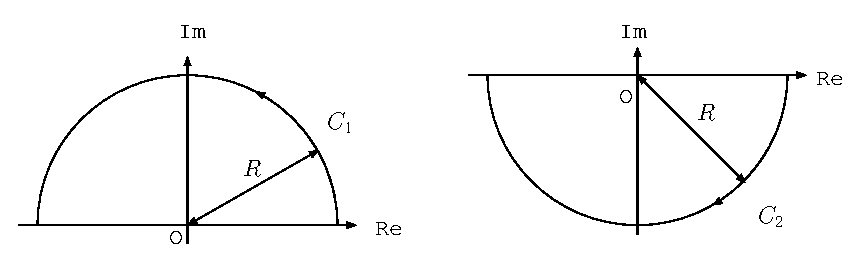
\includegraphics[width=.8\linewidth]{fig/jordan.eps}
  \end{center}
  \caption{
    ジョルダンの補題。$F(z)\e^{ikx}$の積分においては、
    $x$の値によって積分路を変える必要がある。
    $x>0$の場合は$C_1$(上半面)を、$x<0$の場合は$C_2$(下半面)を通る
    積分路を取る。
  }
  \label{fig_jordan}
\end{figure}

%-----------------------------------------------------------------------
\newpage
\section{第九回 ラプラス変換}
%-----------------------------------------------------------------------

\subsection{目的}

ラプラス変換とは何かを学ぶ。ラプラス変換により、微分方程式の
初期値問題が簡単に解けることを理解する。
ラプラス逆変換の公式を複素積分により導けるようにする。

\subsection{解答}

\ans{28}{1}

フーリエ変換の場合と同様に部分積分を行う。ただし、積分が$x=0$からであるため、
$f(0)$などが出てくることに注意。

\begin{eqnarray}
  {\cal L}[f'(x)] &=& \int_0^\infty \diff x f'(x)\e^{-sx} \\
  &=& \left[ -f(x)\e^{-sx} \right]_0^{\infty}  +  s \int_0^\infty \diff x f(x) \e^{-sx}\\
  &=& s {\cal L}[f(x)] + f'(0)
\end{eqnarray}
高次の微分も同様。

\ans{28}{2}

ラプラス変換の定義から、
\begin{equation}
  {\cal L}[\e^{ax }f(x)] = \int_0^\infty \diff x f(x)\e^{-(s-a)x}
\end{equation}
$s-a = s'$と思えば、
\begin{eqnarray}
  {\cal L}[\e^{ax }f(x)] &=& \int_0^\infty \diff x f(x)\e^{-s'x}\\
  &=& \hat{f}(s')\\
  &=& \hat{f}(s-a)
\end{eqnarray}

\ans{28}{3}
\begin{eqnarray}
  {\cal L}[f*g(x)] &=&  \int_{0}^{\infty} \diff x \e^{-sx} \int_{0}^{x} \diff y f(x-y)g(y)
\end{eqnarray}
ここで、積分順序を入れ替える。
\begin{equation}
  \int_0^{\infty} \diff x \int_0^{x} \diff y = \int_0^{\infty} \diff y \int_y^{\infty} \diff x
\end{equation}
に注意すると、
\begin{eqnarray}
  {\cal L}[f*g(x)] &=&  \int_0^{\infty} \diff y \int_y^{\infty} \diff x  \e^{-sx} f(x-y)g(y) \\
  &=& \int_0^{\infty} \diff y g(y) \int_y^{\infty} \diff x  \e^{-sx} f(x-y) \\
  &=& \int_0^{\infty} \diff y g(y) \e^{-py} \int_y^{\infty} \diff x  \e^{-s(x-y)} f(x-y) \\
  &=& \int_0^{\infty} \diff y g(y) \e^{-py} \int_0^{\infty} \diff x'  \e^{-sx'} f(x') \\
  &=& {\cal L}[g] {\cal L}[f]
\end{eqnarray}
ただし、途中で$x-y = x'$とおくことで、二項目の積分を$y$に依存しないようにした。


\ans{29}{1}
ラプラス変換の定義から、
\begin{eqnarray}
  {\cal L}[1] &=& \int_0^{\infty} \e^{-sx} \diff x\\
  &=& \frac{1}{s}
\end{eqnarray}

\ans{29}{2}
\begin{eqnarray}
  {\cal L}[\delta(x)] &=& \int_0^{\infty} \diff x \delta(x) \e^{-sx}\\
  &=& 1
\end{eqnarray}

\ans{29}{3}
\begin{eqnarray}
  {\cal L}[x] &=& \int_0^{\infty}  x \e^{-sx} \diff x\\
  &=& \left[ \frac{x \e^{-sx}}{-s} \right]_0^{\infty} + \frac{1}{s} \int_0^{\infty} \e^{-sx} \diff x\\
  &=& \left[ -\frac{\e^{-sx}}{s^2} \right]_0^{\infty} \\
  &=& \frac{1}{s^2}
\end{eqnarray}

\ans{29}{2}
\begin{eqnarray}
  {\cal L}[\e^{\alpha x}] &=& \int_0^{\infty}  \e^{\alpha x} \e^{-sx} \diff x\\
  &=& \int_0^{\infty}  \e^{-(s-\alpha)x} \diff x\\
  &=& \left[ - \frac{\e^{-(s-\alpha)x}}{s-\alpha}  \right]_0^{\infty}\\
  &=& \frac{1}{s-\alpha}
\end{eqnarray}
ただし、$x \rightarrow \infty$で$\e^{-(s-\alpha)x} \rightarrow 0$で
あるために、${\mathrm Re} s > \alpha$でなくてはならない。

\ans{30}{1}
逆ラプラス変換の定義から、
\begin{equation}
  f(x) = \frac{1}{2 \pi i} \int_{a-i\infty}^{\alpha+i\infty} \diff s \frac{\e^{sx}}{s-\alpha}
\end{equation}
ここで、複素積分を用いるが、$\e^{sx}$があるため、$x$の正負によって
積分範囲を変える必要がある。
$x>0$の時は図$\ref{fig_laplace_int}$の左のように積分路$C$を取ることで、
ジョルダンの補題から円弧の部分の積分の寄与は$0$である。
また、積分路の中には$z=\alpha$が一位の極として含まれるので、
留数定理より
\begin{eqnarray}
  f(x) &=& \frac{1}{2 \pi i} \int_C \diff z \frac{\e^{zx}}{z-\alpha}\\
  &=& \e^{\alpha x}
\end{eqnarray}

$x<0$の場合は逆向きに積分路を取る。このとき、
積分路の中には極が含まれないため、
\begin{equation}
  f(x) = 0
\end{equation}
以上から、
\begin{equation}
  f(x) = \left\{
  \begin{array}{cc}
    0       & \qquad x<0 \\
    \e^{ax} & \qquad x>0
  \end{array}
  \right.
\end{equation}


\begin{figure}[htbp]
  \begin{center}
    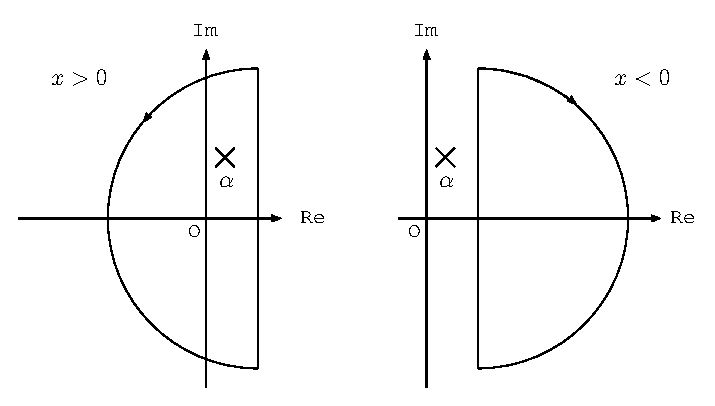
\includegraphics[width=.5\linewidth]{fig/laplace_int.eps}
  \end{center}
  \caption{
    ラプラス逆変換を行うための積分路。
    ジョルダンの補題により、$\e^{sx}$があるため、$x>0$の場合は
    左、$x<0$の場合は右を周る積分路を取らなくてはならない。
    このとき、ラプラス変換が存在する条件は、$s$の実部が
    すべての極の実部よりも大きいことなので、$x<0$の場合は
    必ず$0$となる。
  }
  \label{fig_laplace_int}
\end{figure}

\ans{30}{2}

前問と同様に$x<0$では$f(x) = 0$となるので、$x>0$の場合のみ考える。
\begin{eqnarray}
  f(x) &=& \frac{1}{2 \pi i} \int_C \diff z \frac{z \e^{zx}}{z^2+c^2}
\end{eqnarray}
ここで、特異点は$z = ic, -ic$の二つで、それぞれ一位の極である。
$z = ic$における留数は、
\begin{equation}
  \left. \frac{z \e^{zx}}{z+ic} \right|_{z = ic} = \frac{1}{2}\e^{icx}
\end{equation}
同様に$z = -ic$における留数は、
\begin{equation}
  \left. \frac{z \e^{zx}}{z-ic} \right|_{z = -ic} = \frac{1}{2}\e^{-icx}
\end{equation}
両方足せば、
\begin{equation}
  f(x) = \frac{\e^{icx}+\e^{-icx}}{2} = \cos cx
\end{equation}
を得る。

\ans{31}{1}
微分方程式全体をラプラス変換すると、$f(0)=f'(0)=0$より、
\begin{equation}
  (s^2 - 2s +1) \hat{y}(s) = \frac{1}{s^2}
\end{equation}
すなわち、
\begin{equation}
  \hat{y}(s) = \frac{1}{s^2 (s-1)^2}
\end{equation}
これを部分分数分解すると、
\begin{equation}
  \hat{y}(s) = \frac{-2}{s-1} + \frac{1}{(s-1)^2} + \frac{2}{s} + \frac{1}{s^2}
\end{equation}
ここで、それぞれ
\begin{eqnarray}
  {\cal L}[\e^x] &=& \frac{1}{s-1}\\
  {\cal L}[x\e^x] &=& \frac{1}{(s-1)^2}\\
  {\cal L}[1] &=& \frac{1}{s}\\
  {\cal L}[x] &=& \frac{1}{s^2}
\end{eqnarray}
であるから、
\begin{equation}
  f(x) = -2 \e^{x}+x\e^x+2+x
\end{equation}

微分方程式全体をラプラス変換すると、$f(0)=f'(0)=0$より、
\begin{equation}
  (s^2 + 2s +1) \hat{y}(s) = \frac{1}{s}
\end{equation}
すなわち、
\begin{equation}
  \hat{y}(s) = \frac{1}{s(s+1)^2}
\end{equation}
右辺を部分分数分解する。
やりかたを丁寧に解説すると、
\begin{equation}
  \frac{1}{s(s+1)^2} = \frac{a}{s} + \frac{b}{s+1} + \frac{c}{(s+1)^2}
\end{equation}
と分解できたとすると、両辺に$s$をかけてから$s=0$を代入すれば、
それは$a$である。
すなわち、
\begin{equation}
  a = \left. \frac{1}{(s+1)^2}\right|_{s=0} = 1
\end{equation}
同様に$(s+1)^2$を両辺にかけて$s=-1$を代入すれば、
\begin{equation}
  c = \left. \frac{1}{s}\right|_{s=-1} = -1
\end{equation}
$b$を求めるには、$(s+1)^2$を両辺にかけて微分してから$s=-1$を代入する。
よって、
\begin{equation}
  b = \left. \left(\frac{1}{s}\right)^2 \right|_{s=-1} = -1
\end{equation}
以上より、
\begin{equation}
  \hat{y}(s) =  \frac{1}{s} - \frac{1}{s+1} - \frac{1}{(s+1)^2}
\end{equation}
逆ラプラス変換すれば、
\begin{equation}
  y(x) =  1 - \e^{-x} - x\e^{-x}
\end{equation}
これは確かに$y(0)=y'(0) = 0$であり、
代入すると解になっている。


\subsection{解説}

\subsubsection{ラプラス変換}

フーリエ変換では、関数$f(x)$は無限区間$-\infty < x < \infty$で定義されていた。
変数を時間だと思えば、これは系に安定に存在する解について調べていることになる。
それに対し、電気回路にスイッチを入れたり、バネをはじいたりと、
それまで静的であった系になんらかの刺激を与えたときの応答を知りたい場合が
よくある。そのような過渡的な現象の解析に威力を発揮するのが
{\bf ラプラス変換 (Laplace transform)}である。
過渡的な現象は、微分方程式の初期値問題を解くことに帰着される。
ラプラス変換は、微分方程式の初期値問題を簡単に解く処方箋を与える。

\subsubsection{ラプラス変換とフーリエ変換}

ある関数$f(x)$に対して、次のような関数$g(x)$を考える。
\begin{equation}
  g(x) = \left\{
  \begin{array}{cc}
    0             & \qquad x<0      \\
    \e^{-ax} f(x) & \qquad x \geq 0
  \end{array}
  \right.
\end{equation}

ここで、$g(x)$をフーリエ変換すると、
\begin{eqnarray}
  {\cal F}[g(x)] &=& \int_{-\infty}^{\infty} \diff x g(x) \e^{-ikx}\\
  &=& \int_{0}^{\infty} \diff x \e^{-ax} f(x) \e^{-ikx}\\
  &=& \int_{0}^{\infty} \diff x f(x) \e^{-(a+ik)x}
\end{eqnarray}
ここで、$s = a+ik$とすると、
\begin{eqnarray}
  \int_{0}^{\infty} \diff x f(x) \e^{-(a+ik)x} &=& \int_{0}^{\infty} \diff x f(x) \e^{-sx}\\
  &=& {\cal L}[f(x)]
\end{eqnarray}
これは$f(x)$のラプラス変換に他ならない。
フーリエ変換不可能な関数でも、$a$を十分に大きく取れば$\e^{-ax} f(x)$の
積分が収束し、ラプラス変換が可能である場合がある。
すなわち、ラプラス変換とは、$\e^{-ax}$をかけて収束範囲を広げた
フーリエ変換と考えることができる。

さて、${\cal F}[g(x)]$をフーリエ逆変換しよう。
\begin{eqnarray}
  g(x) &=& \frac{1}{2\pi} \int_{-\infty}^{\infty} \diff k {\cal F}[g(x)] \e^{ikx}\\
  &=& \frac{1}{2\pi} \int_{-\infty}^{\infty} \diff k \hat{f}(s) \e^{ikx}
\end{eqnarray}
ここで、${\cal F}[g(x)] = \hat{f}(s)$であり、$x>0$であれば$g(x) = \e^{-ax} f(x)$であるから、
\begin{eqnarray}
  \e^{-ax} f(x) &=& \frac{1}{2\pi }  \int_{-\infty}^{\infty} \diff k \hat{f}(s) \e^{ikx}\\
  f(x) &=& \frac{1}{2\pi }  \int_{-\infty}^{\infty} \diff k \hat{f}(s) \e^{(a+ik)x}\\
\end{eqnarray}
$s = a + ik$と置くと、$\diff s = i \diff k$、
積分範囲が$a - \infty < s < a + \infty $となることから、
\begin{equation}
  f(x) = \frac{1}{2\pi i}  \int_{a-\infty}^{a+\infty} \diff s \hat{f}(s) \e^{sx}\\
\end{equation}
これは、ラプラス逆変換の定義である。

ここで$a$は 積分
\begin{equation}
  \int_0^{\infty} \e^{-ax} |f(x)| \diff x
\end{equation}
が収束するように選ばれたのであった。これは、$a$が$f(x)$のすべての極よりも
右側にくることを意味する\footnote{ここでは詳細は省略する。参考書を参照のこと}。
これによりラプラス逆変換が$x<0$の時に$f(x)=0$となる。
また、$s = a + ik$とおいたので、${\mathrm Re} s = a$である。
ラプラス変換において、$s$は一般に任意の複素数であるが、その実部は十分に
(ラプラス変換が収束するように)選ばれなければならない。

\subsubsection{非同次方程式とたたみ込み積分}

ラプラス変換は、線形非同次方程式を解くのに威力を発揮する(以下線形を略す)。
非同次方程式とは、次のような形の微分方程式である。
\begin{equation}
  u''(x) + u(x) = f(x) \label{eq_laplace_combo1}
\end{equation}

まず、$f(x)=\delta(x)$と置いた方程式を
\begin{equation}
  v''(x) + v(x) = \delta(x)
\end{equation}
と書こう。この解$v(x)$が得られたとすると、$u$を$v$で表すことができる。
まず、方程式全体をラプラス変換することで、
\begin{equation}
  {\cal L}[v] = \frac{1}{s^2+1} \label{eq_laplace_combo2}
\end{equation}
であることが分かる。
また、式(\ref{eq_laplace_combo1})をラプラス変換すれば、
\begin{equation}
  {\cal L}[u] = \frac{{\cal L}[f]}{s^2+1}\label{eq_laplace_combo3}
\end{equation}
である。式(\ref{eq_laplace_combo2})と式(\ref{eq_laplace_combo3})を見比べれば、
\begin{equation}
  {\cal L}[u] = {\cal L}[v] {\cal L}[f]
\end{equation}
たたみ込み積分のラプラス変換の性質から
${\cal L}[v] {\cal L}[f] = {\cal L}[v*f]$
であるから、
\begin{equation}
  u(x) = \int_0^{x} v(x-y)f(x)  \diff y
\end{equation}
と$u(x)$を$v(x)$で表すことができた。

すなわち、{\bf 同次方程式を解くことができれば、一般の
非同次方程式の解を得ることができる}。

デルタ関数とたたみ込み積分には物理的に重要な関係がある。
過渡的な現象にはたたみ込み積分が現れることが多い。
ある時刻$t=0$にデルタ関数的な刺激を与えたとき、
その出力(応答)が時刻$t$で$w(t)$となるような系を考える。
たとえば、LCR回路に瞬間的に電圧をかけたり、
ぴんと張った弦を弾いたりすると、系はしばらく振動して、
やがて落ち着いていくだろう。
このような応答を{\bf インパルス応答}と呼び、工学では特に重要な概念である。

デルタ関数に対する応答$w(t)$を用いて、任意の入力$f(x)$に対する
出力$h(t)$は
\begin{equation}
  h(t) = \int_0^t w(t-s) f(s) \diff s
\end{equation}
とたたみ込み積分の形で書くことができる。
この式は、時刻$s$での入力$f(s)$が、重み$w(t-s)$で
時刻$t$での出力$h(t)$に影響を与えているという意味を持っている。

%-----------------------------------------------------------------------
\section{おわりに}
%-----------------------------------------------------------------------

以上、物理で使われる数学を一通り学んだ。
かなり駆け足でやったので消化不良のところがあることだろう。
必要に応じて復習して欲しい。その際、教科書を読むだけでなく、
実際に手を動かしてみないと数学は身につかない。
物理で扱う方程式とその解には全て意味がある。
たとえば過渡的な現象であれば$t\rightarrow \infty$で$0$となるはずだろう。
波動方程式の解であれば、なんらかの波を表しているはずだから
周期的な運動を記述するだろう。
問題を解く際にはこのようなイメージを大事にして欲しい。

今回、電磁気学や流体力学で必要となるベクトル解析に
全く触れることができなかった。また、線形代数の扱いは不十分である。
必要であれば各自勉強して欲しい。

\end{document}


